Os valores da \cref{tab:distribuicoes} indicam que a figura \texttt{monalisa.png} foi a que mais sofreu com a mudança de distribuição, enquanto a \texttt{watch.png} quase não teve diferença nas métricas. Isso se deve principalmente ao tamanho da imagem digital, que foram descritos na \cref{sec:intro}. Isso fica mais claro observando os resultados, nas figuras \ref{fig:dist:monalisa} e \ref{fig:dist:watch}.

\begin{figure}[H]
    \centering
    \begin{subfigure}{0.33\textwidth}
    \centering
    \includegraphics[width=4.4cm]{resultados/dists/baboon_floyd.png}
    \caption{Floyd e Steinberg.}
    \label{fig:baboon:floyd}
\end{subfigure}%
\begin{subfigure}{0.33\textwidth}
    \centering
    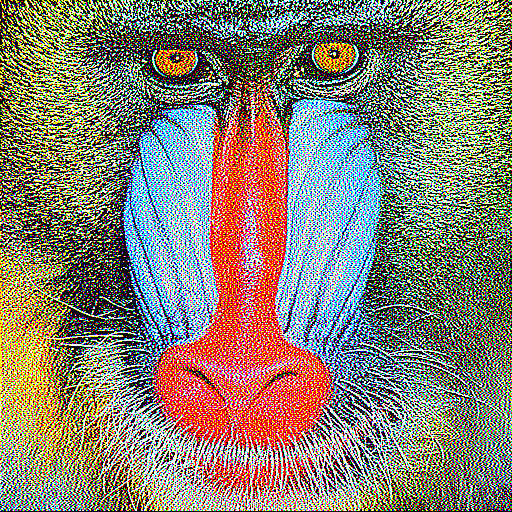
\includegraphics[width=4.4cm]{resultados/dists/baboon_stevenson.png}
    \caption{Stevenson e Arci.}
    \label{fig:baboon:stevenson}
\end{subfigure}%
\begin{subfigure}{0.33\textwidth}
    \centering
    \includegraphics[width=4.4cm]{resultados/dists/baboon_burkes.png}
    \caption{Burkes.}
    \label{fig:baboon:burkes}
\end{subfigure}\\[8pt]
\begin{subfigure}{0.33\textwidth}
    \centering
    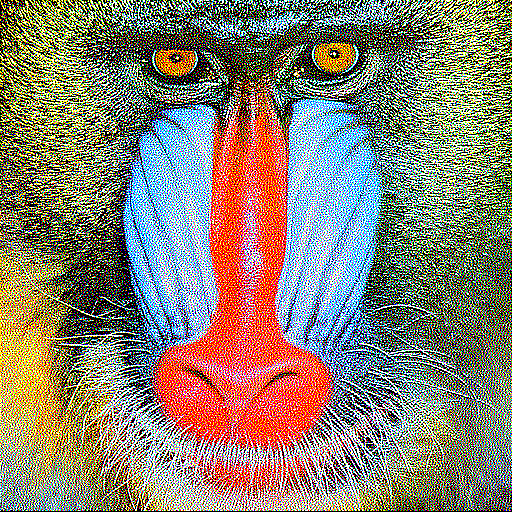
\includegraphics[width=4.4cm]{resultados/dists/baboon_sierra.png}
    \caption{Sierra.}
    \label{fig:baboon:sierra}
\end{subfigure}%
\begin{subfigure}{0.33\textwidth}
    \centering
    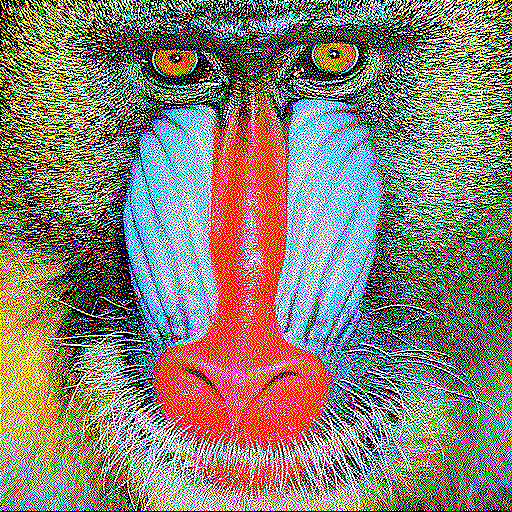
\includegraphics[width=4.4cm]{resultados/dists/baboon_stucki.png}
    \caption{Stucki.}
    \label{fig:baboon:stucki}
\end{subfigure}%
\begin{subfigure}{0.33\textwidth}
    \centering
    \includegraphics[width=4.4cm]{resultados/dists/baboon_jarvis.png}
    \caption{Jarvis, Judice e Ninke.}
    \label{fig:baboon:jarvis}
\end{subfigure}
    \caption{Aplicação das distribuições de erro na \cref{fig:baboon:orig}.}
    \label{fig:dist:baboon}
\end{figure}

Além disso, a diferença entre \texttt{baboon.png} e \texttt{peppers.png}, que têm mesma quantidade de pixels, acontece principalmente por causa das regiões de alta frequência, mais presentes na borda da \texttt{baboon.png}. Essa é a região onde mais se percebe diferenças visuais na \cref{fig:dist:baboon}.

\begin{figure}[H]
    \centering
    \begin{subfigure}{0.33\textwidth}
    \centering
    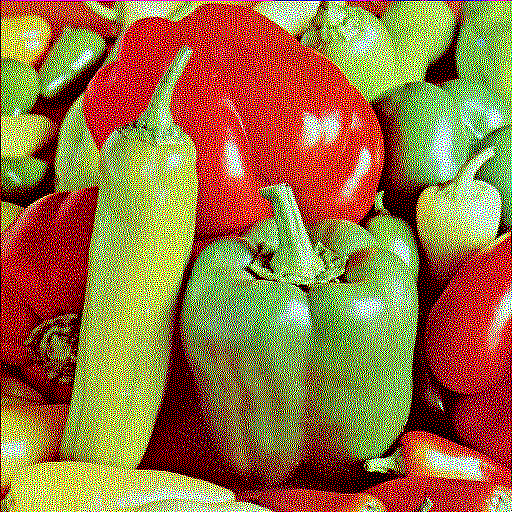
\includegraphics[width=4.4cm]{resultados/dists/peppers_floyd.png}
    \caption{Floyd e Steinberg.}
    \label{fig:peppers:floyd}
\end{subfigure}%
\begin{subfigure}{0.33\textwidth}
    \centering
    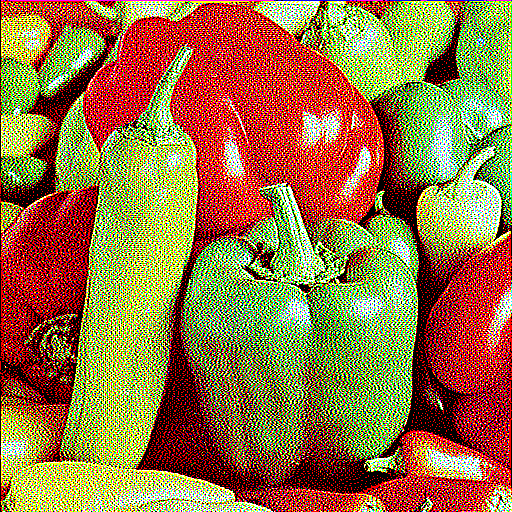
\includegraphics[width=4.4cm]{resultados/dists/peppers_stevenson.png}
    \caption{Stevenson e Arci.}
    \label{fig:peppers:stevenson}
\end{subfigure}%
\begin{subfigure}{0.33\textwidth}
    \centering
    \includegraphics[width=4.4cm]{resultados/dists/peppers_burkes.png}
    \caption{Burkes.}
    \label{fig:peppers:burkes}
\end{subfigure}\\[8pt]
\begin{subfigure}{0.33\textwidth}
    \centering
    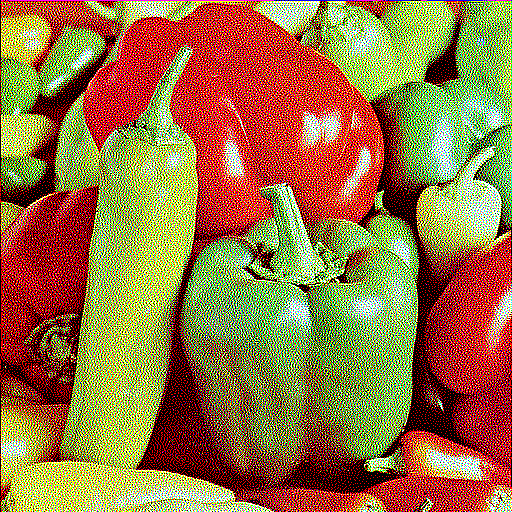
\includegraphics[width=4.4cm]{resultados/dists/peppers_sierra.png}
    \caption{Sierra.}
    \label{fig:peppers:sierra}
\end{subfigure}%
\begin{subfigure}{0.33\textwidth}
    \centering
    \includegraphics[width=4.4cm]{resultados/dists/peppers_stucki.png}
    \caption{Stucki.}
    \label{fig:peppers:stucki}
\end{subfigure}%
\begin{subfigure}{0.33\textwidth}
    \centering
    \includegraphics[width=4.4cm]{resultados/dists/peppers_jarvis.png}
    \caption{Jarvis, Judice e Ninke.}
    \label{fig:peppers:jarvis}
\end{subfigure}
    \caption{Aplicação das distribuições de erro na \cref{fig:peppers:orig}.}
    \label{fig:dist:peppers}
\end{figure}

\begin{figure}[H]
    \centering
    \begin{subfigure}{0.33\textwidth}
    \centering
    \includegraphics[width=4.4cm]{resultados/dists/monalisa_floyd.png}
    \caption{Floyd e Steinberg.}
    \label{fig:monalisa:floyd}
\end{subfigure}%
\begin{subfigure}{0.33\textwidth}
    \centering
    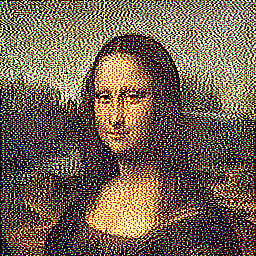
\includegraphics[width=4.4cm]{resultados/dists/monalisa_stevenson.png}
    \caption{Stevenson e Arci.}
    \label{fig:monalisa:stevenson}
\end{subfigure}%
\begin{subfigure}{0.33\textwidth}
    \centering
    \includegraphics[width=4.4cm]{resultados/dists/monalisa_burkes.png}
    \caption{Burkes.}
    \label{fig:monalisa:burkes}
\end{subfigure}\\[8pt]
\begin{subfigure}{0.33\textwidth}
    \centering
    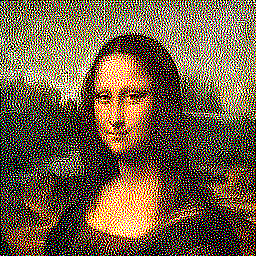
\includegraphics[width=4.4cm]{resultados/dists/monalisa_sierra.png}
    \caption{Sierra.}
    \label{fig:monalisa:sierra}
\end{subfigure}%
\begin{subfigure}{0.33\textwidth}
    \centering
    \includegraphics[width=4.4cm]{resultados/dists/monalisa_stucki.png}
    \caption{Stucki.}
    \label{fig:monalisa:stucki}
\end{subfigure}%
\begin{subfigure}{0.33\textwidth}
    \centering
    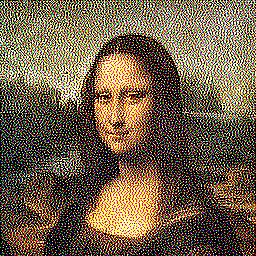
\includegraphics[width=4.4cm]{resultados/dists/monalisa_jarvis.png}
    \caption{Jarvis, Judice e Ninke.}
    \label{fig:monalisa:jarvis}
\end{subfigure}
    \caption{Aplicação das distribuições de erro na \cref{fig:monalisa:orig}.}
    \label{fig:dist:monalisa}
\end{figure}

\begin{figure}[H]
    \centering
    \begin{subfigure}{0.33\textwidth}
    \centering
    \includegraphics[width=4.4cm]{resultados/extra/watch_unidirecional.png}
    \caption{Unidirecional}
    \label{fig:watch:unidirecional}
\end{subfigure}%
\begin{subfigure}{0.33\textwidth}
    \centering
    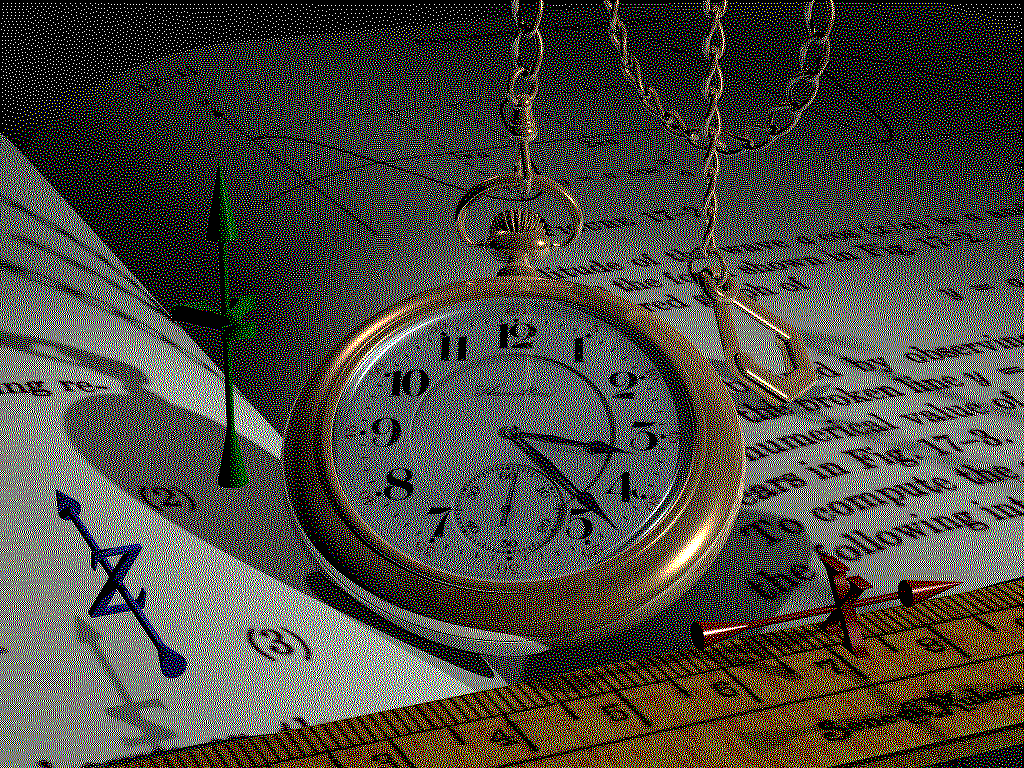
\includegraphics[width=4.4cm]{resultados/extra/watch_alternada.png}
    \caption{Alternada}
    \label{fig:watch:alternada}
\end{subfigure}\\[8pt]
\begin{subfigure}{0.33\textwidth}
    \centering
    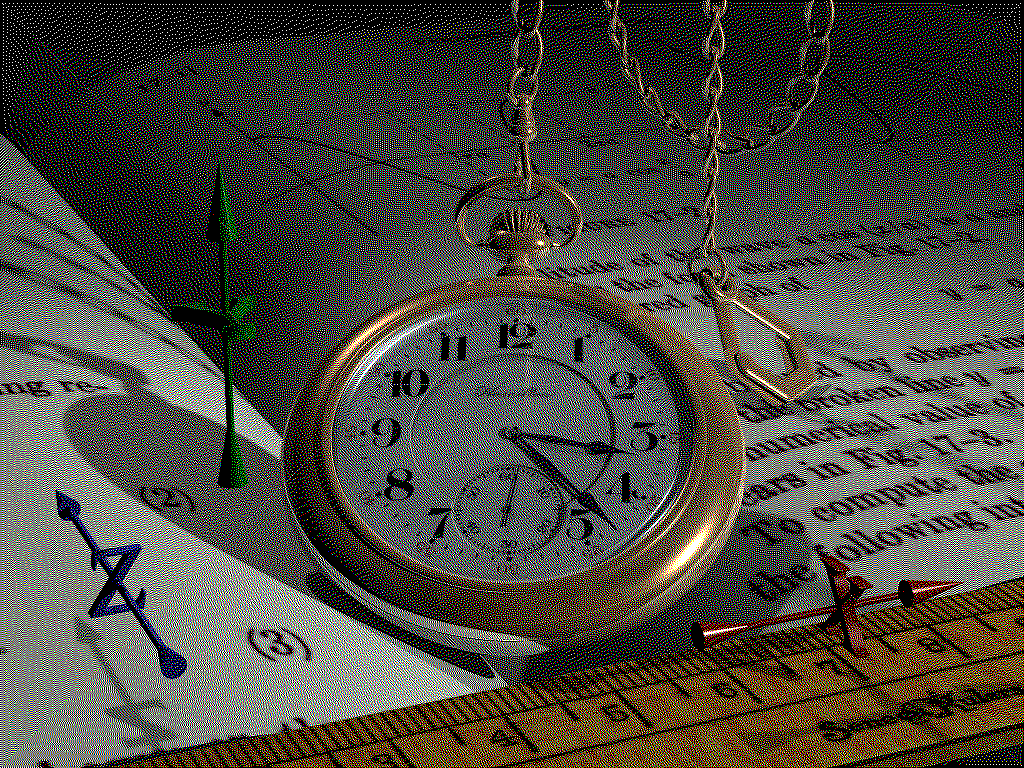
\includegraphics[width=4.4cm]{resultados/extra/watch_espiral.png}
    \caption{Espiral}
    \label{fig:watch:espiral}
\end{subfigure}%
\begin{subfigure}{0.33\textwidth}
    \centering
    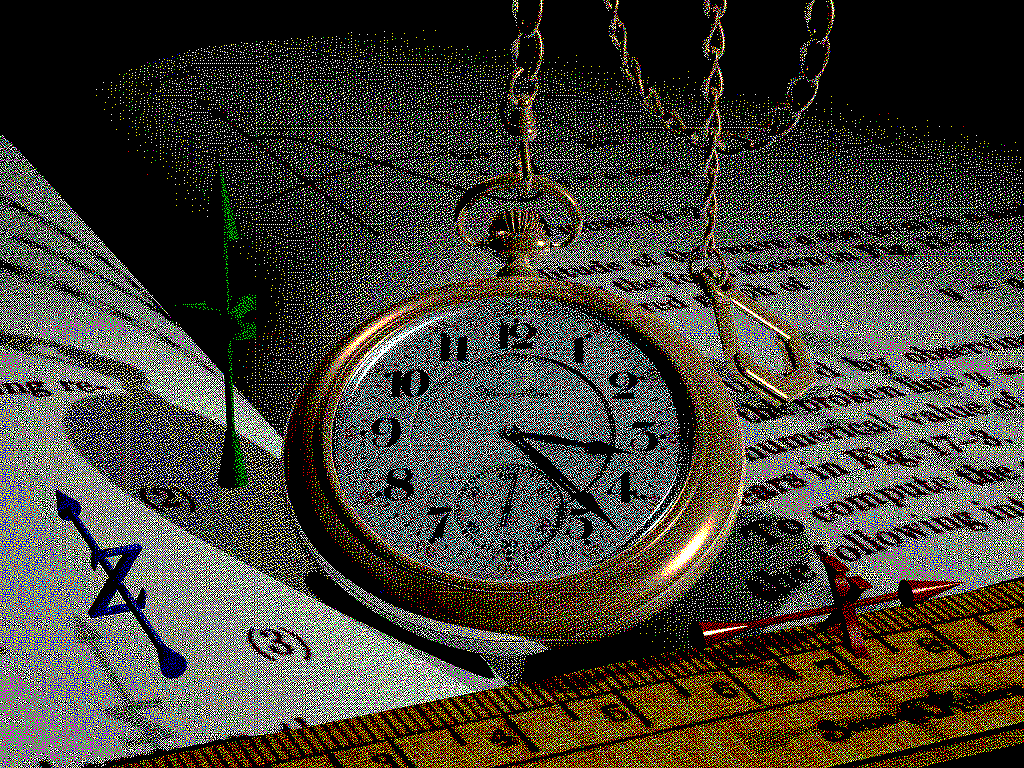
\includegraphics[width=4.4cm]{resultados/extra/watch_hilbert.png}
    \caption{Hilbert}
    \label{fig:watch:hilbert}
\end{subfigure}
    \caption{Aplicação das distribuições de erro na \cref{fig:watch:orig}.}
    \label{fig:dist:watch}
\end{figure}

\begin{table}[H]
    \centering
    \caption{Comparativo entre as distribuições de erros.}
    \label{tab:distribuicoes}
    \begin{tabular}{cc|cccc}
    \toprule
        Figura & Distribuição & RMSE & SNR (dB) & PSNR (dB) & Correlação \\
    \midrule
        \multirow{6}{*}{\texttt{baboon.png}}
        & Floyd e Steinberg & 10.364 & -0.001 & 27.820 & 0.477 \\
        & Stevenson e Arci & 10.367 & -0.003 & 27.818 & 0.578 \\
        & Burkes & 10.365 & -0.002 & 27.819 & 0.512 \\
        & Sierra & 10.364 & -0.001 & 27.820 & 0.547 \\
        & Stucki & 10.369 & -0.005 & 27.816 & 0.540 \\
        & Jarvis, Judice e Ninke & 10.367 & -0.003 & 27.818 & 0.554 \\
    \midrule
        \multirow{6}{*}{\texttt{peppers.png}}
        & Floyd e Steinberg & 10.325 & -0.020 & 27.853 & 0.531 \\
        & Stevenson e Arci & 10.328 & -0.022 & 27.851 & 0.549 \\
        & Burkes & 10.321 & -0.016 & 27.857 & 0.537 \\
        & Sierra & 10.326 & -0.021 & 27.852 & 0.545 \\
        & Stucki & 10.330 & -0.024 & 27.849 & 0.543 \\
        & Jarvis, Judice e Ninke & 10.326 & -0.020 & 27.853 & 0.547 \\
    \midrule
        \multirow{6}{*}{\texttt{monalisa.png}}
        & Floyd e Steinberg & 10.407 & 0.013 & 27.784 & 0.418 \\
        & Stevenson e Arci & 10.411 & 0.009 & 27.781 & 0.443 \\
        & Burkes & 10.412 & 0.008 & 27.780 & 0.422 \\
        & Sierra & 10.415 & 0.006 & 27.777 & 0.433 \\
        & Stucki & 10.413 & 0.008 & 27.780 & 0.428 \\
        & Jarvis, Judice e Ninke & 10.406 & 0.013 & 27.785 & 0.435 \\
    \midrule
        \multirow{6}{*}{\texttt{watch.png}}
        & Floyd e Steinberg & 10.263 & 0.015 & 27.905 & 0.371 \\
        & Stevenson e Arci & 10.263 & 0.015 & 27.906 & 0.392 \\
        & Burkes & 10.264 & 0.014 & 27.905 & 0.374 \\
        & Sierra & 10.265 & 0.013 & 27.904 & 0.379 \\
        & Stucki & 10.264 & 0.015 & 27.905 & 0.379 \\
        & Jarvis, Judice e Ninke & 10.264 & 0.014 & 27.905 & 0.380 \\
    \bottomrule
\end{tabular}

\end{table}
